\documentclass{article}
\usepackage[preprint]{tmlr}
\usepackage[utf8]{inputenc}
\usepackage[T1]{fontenc}
\usepackage{amsmath,amssymb}
\usepackage{booktabs}
\usepackage{hyperref}
\usepackage{xcolor}
\usepackage{graphicx}
\usepackage{multirow}
\newtheorem{proposition}{Proposition}
\newtheorem{corollary}[proposition]{Corollary}

\title{Fishing for Privacy: Machine Unlearning for Single-Cell VAEs}

\author{\name David Benson \email dmb2262@columbia.edu \\
        \addr Columbia University}

\begin{document}

\maketitle

\begin{abstract}
Variational autoencoders trained on gene-expression data memorize rare biological subpopulations, and those are the samples where a membership inference attack (MIA) is most dangerous. A few patients with an unusual disease subtype, or a small cluster of rare cells, can be individually identifiable from model behavior. Can such memorization be selectively removed without retraining the model, and without destroying its utility? That requires fixing the measurement first. MIA protocols that draw matched negatives from different biological classes than the forget set can conflate subtype identity with training membership, and this confound affects general-purpose attacks (threshold, likelihood ratio, $k$-NN) along with the distance-based methods used in recent transcriptomics benchmarks. A trained MLP attacker on model-internal features, evaluated against a multi-seed retrain baseline under the identical matched-negative protocol, recovers a smaller memorization signal that sits almost entirely in biologically coherent subpopulations; within-subtype matching corroborates this where enough held-out cells of the forget class exist. The three cohorts play different roles under this evaluation. On Tabula Muris and TCGA-BRCA the retrain reference meets or exceeds the baseline, so no membership signal is present to unlearn, which is itself informative. On PBMC-33k, where a genuine signal survives, no post-hoc method reliably reaches retrain-level privacy across seeds and forget-set sizes. Methods that preserve utility produce no privacy improvement. The methods that do reduce the membership signal destroy the model through posterior collapse or Streisand effects~\citep{hayes2024}. The underlying cause is structural. Fisher information overlap in the VAE's shared decoder output layer is roughly $27\times$ higher between forget and retain sets than in a classifier's class-specific output ($0.48$ vs.\ $0.018$ under a per-sample estimator), and Proposition~\ref{prop:factorization} formalizes why. With $D$ shared output dimensions the overlap grows as $1 - O(M/D)$, while a classifier's class-specific heads give overlap $O(1/\sqrt{C})$. If privacy actually matters, retrain.
\end{abstract}

\section{Introduction}

Deep learning models memorize training data, and for rare subpopulations this memorization may be necessary for generalization~\citep{feldman2020}. When those models are trained on sensitive biological information, an attacker can determine whether a specific sample was part of the training set through a membership inference attack (MIA). Gene expression profiles can reveal disease status, genetic predispositions, and other personal health information. Rare cell types and disease subtypes may be individually identifiable even within large, aggregated datasets.

Can a gene-expression VAE selectively forget a rare biological subpopulation without retraining and without destroying model utility? This question arises when all cells from a specific cluster or all patients of a molecular subtype must be removed from a trained model. Experiments here use cell-type clusters (PBMC-33k, Tabula Muris) and disease subtypes (TCGA-BRCA) as forget sets across two modalities (single-cell and bulk RNA-seq).

Before testing unlearning methods, the evaluation itself had to be fixed. MIA protocols that draw matched negatives from different biological classes than the forget set can conflate subtype identity with training membership. This affects general-purpose attacks (threshold~\citep{yeom2018}, likelihood ratio~\citep{carlini2022}, $k$-NN~\citep{shokri2017}) as well as the distance-based methods used in recent transcriptomics benchmarks~\citep{ozturk2026, golob2026}. Within-subtype matching, a trained MLP attacker on model-internal features, and a multi-seed retrain baseline together isolate the genuine memorization signal, which concentrates in biologically coherent subpopulations.

Under this corrected evaluation, PBMC-33k is the one cohort with a genuine membership signal, and there no post-hoc method reliably reaches retrain-level privacy; on Tabula Muris and TCGA-BRCA no signal is present to unlearn. Methods that preserve utility produce no privacy improvement. Methods that reduce the membership signal destroy the model through posterior collapse or Streisand effects, where the act of unlearning leaves a detectable trace that makes forget-set samples more distinguishable than before~\citep{hayes2024}. The cause is Fisher information overlap in the VAE's shared decoder, which prevents selective parameter perturbation.

\paragraph{Contributions.}
\begin{enumerate}
    \item A corrected evaluation protocol for MIA on biological generative models. Cross-class matched-negative protocols can conflate cell-type identity with training membership. The operative correction for the main results is a multi-seed retrain baseline evaluated under the identical matched-negative protocol together with a trained attacker on model-internal features; within-subtype matching corroborates it where enough held-out cells of the forget class exist. These isolate the genuine memorization signal, which concentrates in biologically coherent subpopulations. The confound magnitude varies by dataset and is documented per-dataset in Section~\ref{sec:confound}.

    \item A systematic evaluation of eleven unlearning approaches (nine approximate methods plus training-time synthetic augmentation and representation alignment) across three datasets and two modalities. The unlearning failure is established on PBMC-33k, the one cohort with a measurable membership signal, where methods either fail to reduce the signal or reduce it but destroy model utility. On scattered forget sets memorization is negligible and unlearning is unnecessary. On Tabula Muris and TCGA-BRCA the retrain reference meets or exceeds the baseline, so no membership signal is present to unlearn under the tested attack suite.

    \item A structural explanation via Fisher information overlap. The VAE's shared decoder output layer creates roughly $27\times$ higher Fisher alignment between forget and retain sets than a classifier's class-specific output ($0.485$ vs.\ $0.018$ on PBMC; $0.75$ on TCGA-BRCA), while the global-parameter cosine ($0.21$) still gives an $11\times$ gap. Proposition~\ref{prop:factorization} formalizes this for linear decoders, with dimensional scaling bounds showing generative-model overlap grows as $1 - O(M/D)$ while classifier overlap scales as $1/\sqrt{C}$.
\end{enumerate}

\begin{figure*}[t]
  \centering
  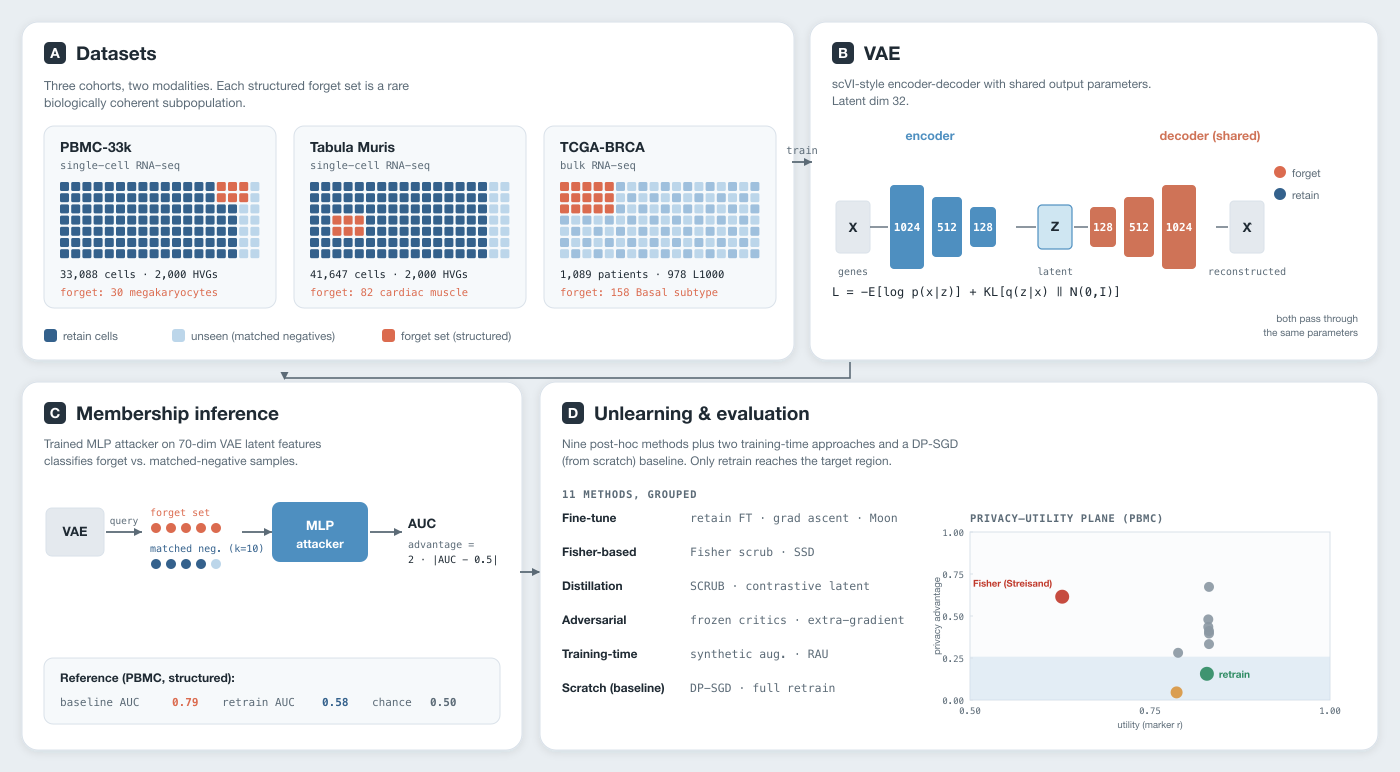
\includegraphics[width=0.95\textwidth]{figures/eval_pipeline.pdf}
  \caption{Evaluation pipeline. \textbf{(A)} Three cohorts across two modalities, each with a structured forget set that is a rare, biologically coherent subpopulation. \textbf{(B)} scVI-style VAE, latent dim 32. \textbf{(C)} A trained MLP attacker on 70-dim latent features classifies forget versus matched-negative samples; matched negatives are drawn within-subtype via $k$-nearest neighbors. \textbf{(D)} Eleven unlearning approaches (nine post-hoc, two training-time) plus DP-SGD on the privacy--utility plane; no post-hoc method reaches the target (advantage $\leq 0.258$, the $95\%$ CI upper bound of the retrain baseline), which only full retraining and from-scratch DP-SGD attain.}
  \label{fig:pipeline}
\end{figure*}

\section{Background and threat model}

\paragraph{Unlearning and MIA.} Machine unlearning produces parameters $\theta'$ from a trained model, forget set $\mathcal{F}$, and retain set $\mathcal{R} = \mathcal{D} \setminus \mathcal{F}$ such that a post-hoc MIA cannot distinguish forget samples from never-seen samples~\citep{cao2015, bourtoule2021}. Theoretical guarantees exist for restricted model classes~\citep{ginart2019, guo2020, sekhari2021, neel2021, izzo2021} but depend on convexity or smoothness that deep generative models violate. MIA determines training-set membership via shadow models~\citep{shokri2017} or likelihood ratios~\citep{carlini2022}. Privacy leakage is reported as membership inference advantage (adapted from~\citet{yeom2018}): $\text{advantage} = 2|\text{AUC} - 0.5|$, direction-agnostic because an adversary can always flip predictions. \citet{hayes2024} showed that inexact unlearning can leave forgotten samples more detectable (Streisand effect); \citet{thudi2022} argued that without auditable definitions, unlearning claims are unverifiable.

\paragraph{Threat model.} The scope is subpopulation unlearning, the removal of entire biological groups (rare cell types, disease subtypes) rather than individual samples. Data poisoning, adversarial extraction, and reconstruction attacks are out of scope. The adversary has query access and trains a dedicated attacker on data they control, which is a stronger setting than off-the-shelf distance-based MIA such as GAN-leaks~\citep{ganleaks2020}, Monte Carlo, or Mahalanobis distance. A model that faithfully captures subtype biology will by construction produce outputs close to real training members of the same subtype, yielding high MIA scores that reflect biological fidelity rather than memorization. The trained MLP attacker used here (70-dim features from the VAE latent space) learns which feature combinations are informative for membership specifically, as evidenced by its near-chance retrain advantage ($0.16$) compared to distance-based methods (advantage $\geq 0.43$ on the retrain model; Table~\ref{tab:attacks}).

\paragraph{Related work.} Fisher scrubbing~\citep{golatkar2020}, SSD~\citep{foster2024}, and SCRUB~\citep{kurmanji2023} all assume forget-set influence concentrates in identifiable parameter subsets, an assumption Section~\ref{sec:fisher} shows breaks down in shared-decoder architectures. \citet{nasr2018} and~\citet{chavdarova2019} provide the adversarial min-max and extragradient machinery used in extra-gradient co-training; \citet{abadi2016} introduced DP-SGD, used here as a formal privacy baseline. \citet{moon2024} proposes feature unlearning for pre-trained generators by fine-tuning the decoder along a target-feature latent direction, evaluated here as a post-hoc method (Table~\ref{tab:methods}). \citet{cheng2026} studies retain-forget entanglement in classifiers via Wasserstein regularization, without a Fisher-overlap account; the present work locates the entanglement structurally in the shared decoder output of a generative model and formalizes it (Proposition~\ref{prop:factorization}), showing it defeats unlearning precisely where a classifier's class-specific outputs avoid it. On biological data, \citet{walker2024} showed single-cell count matrices leak private information via eQTL linkage. \citet{golob2026} introduced scMAMA-MIA for scRNA synthetic data and observed per-cell-type vulnerability but set it aside as out of scope; \citet{ozturk2026} reported $\rho = 0.92$ between differential expression recovery and MIA vulnerability across 11 generative models on TCGA. Both use distance-based MIA on synthetic outputs and do not stratify by subtype. \citet{lopez2018} developed scVI, the architecture tested here.

\section{Datasets and setup}
\label{sec:datasets}

Figure~\ref{fig:pipeline} summarizes the full evaluation pipeline. This section describes the datasets and the forget-set construction, and Section~\ref{sec:confound} develops the within-subtype evaluation protocol.

\begin{table}[t]
\centering
\caption{Dataset and split summary. Matched negatives are the $k$-nearest unseen samples to the structured forget set in baseline latent space ($k=10$). TCGA-BRCA data from~\citet{ozturk2026}, VST-normalized, 978 LINCS L1000 landmark genes~\citep{subramanian2017}.}
\label{tab:datasets}
\begin{tabular}{lccc}
\toprule
 & PBMC-33k & Tabula Muris & TCGA-BRCA \\
\midrule
Type & scRNA-seq & scRNA-seq & Bulk RNA-seq \\
Samples & 33,088 cells & 41,647 cells & 1,089 patients \\
Genes & 2,000 HVGs & 2,000 HVGs & 978 L1000 \\
Train / Unseen & 28,124 / 4,964 & 35,399 / 6,248 & 925 / 164 \\
Structured forget & Cluster 13 (30 megakaryocytes) & Cluster 33 (82 cardiac muscle) & Basal subtype (158 patients) \\
Forget fraction & 0.1\% & 0.2\% & 17\% \\
Patient-level forget & N/A & N/A & 5, 10, 20 patients \\
Matched negatives & 194 & 137 & 121 \\
\bottomrule
\end{tabular}
\end{table}

The PBMC-33k dataset consists of 33,088 peripheral blood mononuclear cells from 10x Genomics, preprocessed with Scanpy~\citep{wolf2018}, each represented by 2,000 highly variable gene counts. The structured forget set is cluster 13, which contains 30 rare megakaryocytes. The Tabula Muris dataset~\citep{tabula2018} has 41,647 cells from 12 mouse tissues with 35 Leiden clusters; the structured forget set is cluster 33 (82 cardiac muscle cells). The TCGA-BRCA dataset~\citep{tcga2012} consists of 1,089 breast cancer patients with PAM50 molecular subtypes (LumA 52\%, LumB 20\%, Basal 17\%, Her2 8\%, Normal 4\%), preprocessed by~\citet{ozturk2026} for the CAMDA 2025 Health Privacy Challenge. Each sample corresponds to one patient, enabling patient-level forget sets. Table~\ref{tab:datasets} gives a full comparison.

To control for biological confounds in MIA evaluation, matched negatives were selected as the unseen cells closest to the forget set in the baseline model's latent space ($k$-NN with $k=10$). Without this control, an attacker could distinguish forget from unseen cells by cell type alone rather than by memorization. A within-subtype holdout variant restricts matched negatives to the same biological group as the forget set. On PBMC, this drops baseline AUC from 0.769 to 0.527 (5 unseen megakaryocytes); on TCGA-BRCA, baseline and retrain AUCs converge to 0.576 (30 unseen Basal patients). Section~\ref{sec:confound} quantifies this confound across datasets.

\section{Methods}
\label{sec:methods}

\subsection{VAE architecture}

The VAE follows scVI design principles~\citep{lopez2018}. The encoder maps input genes (2,000 for PBMC/Tabula Muris; 978 for TCGA-BRCA) through layers $[1024, 512, 128]$ to latent mean $\mu$ and log-variance $\log\sigma^2$ with latent dimension 32. The decoder reverses this through $[128, 512, 1024]$ to a softmax output across genes. Layer normalization and dropout (0.1) follow each hidden layer. Because the input data are log-normalized (Section~\ref{sec:datasets}), the reconstruction term is mean squared error (Gaussian observation model on the transformed counts); the training objective is the negative ELBO, $\mathcal{L}(\theta, \phi; x) = -\mathbb{E}_{q_\phi(z|x)}[\log p_\theta(x|z)] + \text{KL}(q_\phi(z|x) \| p(z))$.

\subsection{Unlearning methods}

Nine post-hoc approximate unlearning methods were tested, alongside DP-SGD~\citep{abadi2016} as a formal privacy baseline that trains from scratch on the retain set. Full hyperparameters and pseudocode are in the released code; the summary below names each approach and cites its origin. \textbf{Retain-only fine-tuning} continues VAE training on $\mathcal{R} = \mathcal{D} \setminus \mathcal{F}$. \textbf{Gradient ascent} maximizes forget-set loss then fine-tunes on the retain set. \textbf{Frozen critics} freeze pre-trained MIA attackers and update the VAE to minimize critic success. \textbf{Fisher information scrubbing}~\citep{golatkar2020} updates $\theta \leftarrow \theta + \alpha(F + \lambda I)^{-1}\nabla_\theta \mathcal{L}_\mathcal{F}$ with the diagonal Fisher information $F$ on the forget set. \textbf{SSD}~\citep{foster2024} dampens parameters multiplicatively in proportion to forget-set Fisher importance. \textbf{SCRUB}~\citep{kurmanji2023} uses teacher-student distillation that matches on retain data and diverges on forget data. \textbf{Moon feature unlearning}~\citep{moon2024} builds a forget-versus-retain latent direction and fine-tunes the decoder so forget-set latents reconstruct with that direction removed while retain reconstructions are preserved, leaving the encoder fixed. \textbf{Contrastive latent unlearning} pushes forget-set posteriors toward the prior $\mathcal{N}(0, I)$ while preserving retain-set representations. \textbf{Extra-gradient co-training} frames unlearning as a min-max game,
\begin{equation}
\min_\theta \max_\psi \mathcal{L}_{\text{VAE}}(\theta; \mathcal{R}) - \lambda \cdot \mathcal{L}_{\text{att}}(\theta, \psi; \mathcal{F}),
\end{equation}
and uses the two-step extragradient update of~\citet{chavdarova2019} with TTUR (attacker LR $10\times$ lower than VAE LR), three co-trained critics, and 50 epochs (stopping before equilibrium). Hyperparameters for each method were chosen by sweep on PBMC-33k; results below report multi-seed evaluation at the chosen settings.

\subsection{Attack suite}

The canonical attacker is a trained MLP on 70-dimensional features (69 VAE latent statistics plus a $k$-NN distance to the retain set, $k=5$; spectral normalization, two hidden layers of 256, dropout 0.3). A single attacker is trained on the baseline model's forget-versus-matched-negative features, where the membership signal is strongest, and then applied unchanged to every target model, including each unlearned checkpoint and the retrain reference. This fixed decision rule is if anything more lenient than an attacker refit to each model, so the finding that every post-hoc method still fails against it is conservative; the same attacker scores the retrain reference near chance, which calibrates the measurement and shows the rule is tuned to membership rather than to a per-model boundary refit to noise. Three additional attack families provide robustness checks. \textbf{Threshold attacks} apply a threshold to reconstruction loss, KL divergence, or ELBO individually~\citep{yeom2018} and require only black-box access. \textbf{Likelihood-ratio} compares per-sample loss under the target model against the retrain reference~\citep{carlini2022}. \textbf{$k$-NN latent} classifies membership by distance to known training samples in latent space ($k=10$)~\citep{shokri2017}.

The evaluation target is a 5-seed retrain baseline (seeds 42--46), yielding fresh-attacker advantage $0.16$ with an exact nested $95\%$ CI $[0.08, 0.26]$ (AUC $= 0.578$) that combines cross-seed variance with within-eval bootstrap uncertainty on the $\approx 224$-sample matched-negative pool. Every method carries the same nested CI, and each is compared to retrain by a nested bootstrap of the advantage difference rather than a test on seed means alone. A permutation null with no membership signal present sets the advantage estimator's floor at $0.091$ ($95\%$ $[0.003, 0.253]$), so the retrain reference itself sits only marginally above chance, consistent with the biology confound. The per-method advantage is the mean across seeds of the folded per-seed value $2|\mathrm{AUC}_s - 0.5|$; for high-variance methods this exceeds $2|\overline{\mathrm{AUC}} - 0.5|$ (extra-gradient reports $0.281$ against $0.134$ from the mean AUC of $0.433$), which is why the permutation floor calibrates the estimator and why extra-gradient's advantage CI $[0.20, 0.37]$ overlapping that floor is the honest reading of its result.

\section{The biology confound}
\label{sec:confound}

On TCGA-BRCA (1,089 breast cancer patients, bulk RNA-seq), the structured forget set is 158 Basal-subtype patients (17\% of training). With standard cross-subtype matching, baseline AUC $= 0.821$ and retrain AUC $= 0.860$. The retrain model, which never saw the Basal patients, is better at detecting them than the baseline. All six tested unlearning methods converge to the retrain floor ($\text{AUC} \approx 0.862$).

Within-subtype matching (restricting matched negatives to 30 unseen Basal patients) resolves the cross-subtype confound. Baseline and retrain advantages both reach $\approx 0.15$ and become indistinguishable from each other. The entire cross-subtype gap was driven by Basal identity. The residual within-subtype advantage of $0.15$ is not zero, so the attacker still detects something, but whatever it detects is equally present in the retrain model that never saw the Basal patients, and is therefore not a membership signal. Patient-level experiments at $n_f \in \{5, 10, 20\}$ show the same pattern: baseline and retrain advantages overlap within their CIs at every size, with no consistent gap.

The confound replicates on PBMC. Within-cluster matching (5 unseen megakaryocytes) drops baseline AUC from 0.769 to 0.527 while retrain rises from 0.495 to 0.609, indicating that most of the cross-cluster above-chance signal is attributable to subtype identity rather than memorization. Replication on PBMC cluster 7 (CD14+ monocytes, 80 unseen cells) shows a similar pattern (cross-cluster AUC $= 0.665$, within-cluster AUC $= 0.527$), removing the dependence on a 5-cell holdout. Tabula Muris cluster 28 (67 unseen) shows no detectable per-sample memorization under either matching strategy. Table~\ref{tab:attacks} shows the confound at the attack level: high-assumption attacks ($k$-NN, likelihood ratio) achieve advantage $\geq 0.73$ on the retrain model because they detect biological structure regardless of training history.

A second rare cluster confirms both the confound and the unlearning failure. PBMC cluster 12 (49 cells) has baseline AUC $0.87$ (advantage $0.73$), yet a model retrained without those cells still reaches AUC $0.82$ (advantage $0.64$), so the genuine membership gap is only $\approx 0.09$ and a biology confound carries the rest, a smaller gap than cluster 13's $0.21$. Against this second forget set no post-hoc method reaches the retrain reference while preserving utility. Retain-only fine-tuning holds advantage at the baseline level ($0.72$, marker correlation $0.83$), Fisher scrubbing again collapses the posterior (marker correlation falls to $0.34$), and the extra-gradient configuration ($\lambda = 10$) that reaches the retrain floor on cluster 13 over-unlearns here, driving advantage to $0.00$ while degrading marker correlation to $0.76$. The one method competitive on cluster 13 is therefore not robust to the choice of forget set, and the failure is not an artifact of a single cluster.

Figure~\ref{fig:confound} in Appendix~\ref{app:confound} visualizes the cross-subtype vs.\ within-subtype comparison and decomposes the cross-subtype AUC into biology and memorization components.

The confound is consistent with two recent benchmarks that report high MIA scores on scRNA and bulk RNA using distance-based MIA on synthetic outputs. \citet{ozturk2026} report $\rho = 0.92$ between differential expression recovery and MIA vulnerability across 11 generative models (TCGA-COMBINED, $n = 11$ so the correlation is suggestive), and \citet{golob2026} observe cell-type-dependent vulnerability in scMAMA-MIA but set the dependence aside as out of scope. Distance-based methods on synthetic outputs cannot distinguish biological signal preservation from individual-level memorization; a trained MLP attacker on model-internal features can, as its lower retrain advantage ($0.16$) compared to baseline ($0.58$) on PBMC shows.

\section{Unlearning results}

\subsection{Unlearning methods on structured forget set}

\begin{table}[t]
\centering
\caption{All methods on PBMC-33k structured forget set (cluster 13, $n=30$), from the per-seed evaluation with a fresh canonical attacker. Advantage carries an exact nested $95\%$ CI combining cross-seed and within-eval ($\sim$224-sample) bootstrap uncertainty. Status is set by comparing the per-seed advantage to the retrain $95\%$ CI upper bound ($0.258$) and by a nested bootstrap of the method-minus-retrain advantage difference. Every post-hoc method exceeds the bound, and every post-hoc difference CI excludes zero except extra-gradient, whose difference from retrain is not resolved while its point advantage still exceeds the bound. Under a permutation null with no membership signal present, the advantage estimator itself reports $0.091$ ($95\%$ $[0.003, 0.253]$), so values near this floor are not distinguishable from chance. $\dagger$Single-checkpoint entries carry within-eval CIs only and are excluded from the difference test. AUCs here are multi-seed means; the single-run canonical attacker used in Sections~\ref{sec:confound} and~\ref{sec:crossdataset} reports baseline $0.769$ and retrain $0.481$ on one fixed checkpoint pair.}
\label{tab:methods}
\begin{tabular}{lccccc}
\toprule
Method & Seeds & AUC & Advantage [95\% CI] & Marker $r$ & Status \\
\midrule
Baseline (no unlearning) & 1 & 0.791 & 0.582 & 0.831 & anchor \\
\midrule
Retain-only fine-tune & 5 & 0.666 & 0.333 [0.23, 0.43] & 0.832 & FAIL \\
Gradient ascent & 5 & 0.698 & 0.396 [0.30, 0.49] & 0.832 & FAIL \\
SSD ($\alpha=1.0$) & 3 & 0.718 & 0.435 [0.31, 0.56] & 0.831 & FAIL \\
SCRUB ($\alpha_f=1.0$) & 3 & 0.706 & 0.411 [0.28, 0.54] & 0.832 & FAIL \\
Moon feature-unlearn & 3 & 0.740 & 0.480 [0.36, 0.60] & 0.831 & FAIL \\
Contrastive latent ($\gamma=1.0$) & 3 & 0.164 & 0.673 [0.57, 0.75] & 0.832 & FAIL (Streisand) \\
Fisher scrubbing$^\dagger$ & 1 & 0.808 & 0.615 [0.45, 0.77] & -- & FAIL (worse) \\
Frozen critics$^\dagger$ ($\lambda=10$) & 1 & 0.992 & 0.984 & -- & FAIL \\
Extra-grad ($\lambda=10$) & 10 & 0.433 & 0.281 [0.20, 0.37] & 0.789 & FAIL (marginal) \\
\midrule
DP-SGD ($\varepsilon=10$) & 3 & 0.478 & 0.045 [0.03, 0.18] & 0.787 & $\approx$ retrain$^{*}$ \\
Full retrain & 5 & 0.578 & 0.156 [0.08, 0.26] & 0.829 & TARGET \\
\bottomrule
\end{tabular}
\end{table}

Table~\ref{tab:methods} groups the nine post-hoc methods by failure mode alongside the DP-SGD baseline.

\paragraph{Utility-preserving, privacy-failing.} Retain-only fine-tuning, gradient ascent, SSD, and SCRUB preserve utility (marker $r \geq 0.831$) but produce no useful privacy reduction, with advantages of $0.33$ to $0.44$. Thirty forget-set cells leave too small a gradient signal against the 28,094 retain cells. Each has a method-minus-retrain advantage difference whose nested $95\%$ CI excludes zero (probability above retrain $\geq 0.99$). SSD at $\alpha = 5.0$ (single seed) lowers advantage to $0.27$, still above the retrain CI upper bound ($0.26$).

\paragraph{Detectable artifacts.} Three methods make the model worse rather than better. Contrastive latent unlearning drops AUC to $0.164$ (advantage $= 0.673$), a Streisand effect~\citep{hayes2024} where the forced move to the prior is itself a detectable signature. Fisher scrubbing collapses the posterior (KL falls from $10.55$ to $0.007$) and advantage rises to $0.615$. Frozen critics (AUC $= 0.992^\dagger$) exploit fixed decision boundaries without removing the underlying signal.

\paragraph{Adversarial and formal.} Extra-gradient with $\lambda = 10$ (10 seeds) reduces mean advantage to $0.281$ but with $\sigma_{\text{AUC}} = 0.142$; per-seed behavior spans over- and under-unlearning, and its advantage difference from retrain is not statistically resolved (nested $95\%$ CI $[-0.01, 0.24]$ includes zero, probability above retrain $0.97$), so it is the single method whose separation from retrain is not established, though its point advantage still exceeds the retrain CI upper bound ($0.258$). The method fails outright on Tabula Muris (Section~\ref{sec:crossdataset}) and over-unlearns on a second PBMC forget set, where the same $\lambda = 10$ drives advantage to $0.00$ at a utility cost rather than reaching the target (Section~\ref{sec:confound}), so the configuration does not transfer across forget sets. DP-SGD at $\varepsilon = 10$ reaches advantage $= 0.045$, and its difference from retrain is not distinguishable from zero (nested $95\%$ CI $[-0.19, 0.04]$), but it is not unlearning; the forget set was never in training, and ELBO rises from $364$ to $403$ while marker $r$ drops from $0.831$ to $0.787$. The $^*$ in Table~\ref{tab:methods} marks this distinction.

Fisher behaves differently across forget-set types. On scattered forget sets it achieves AUC $= 0.499$ (near chance) but from a baseline of $0.525$, so the actual privacy gain is $\Delta = 0.026$; on structured sets it collapses the posterior and makes privacy worse. The one method that works on scattered sets fails where memorization is strongest (full ablation in Appendix~\ref{app:fisher_scattered}).

\subsection{Attack diversity}

\begin{table}[t]
\centering
\caption{Attack suite results on PBMC-33k structured forget set. Advantage $= 2|\text{AUC} - 0.5|$. Low-assumption attacks use only loss components; high-assumption attacks require a reference model or training set embeddings. The trained MLP (canonical attacker) is shown for comparison.}
\label{tab:attacks}
\begin{tabular}{llcccc}
\toprule
 & Attack & Baseline & Retrain & EG $\lambda$=10 & Fisher \\
\midrule
\multirow{3}{*}{\rotatebox{90}{\small Low}} & Recon.\ threshold & 0.438 & 0.438 & 0.438 & 0.438 \\
 & KL threshold & 0.841 & 0.733 & 0.192 & 0.272 \\
 & ELBO threshold & 0.838 & 0.725 & 0.023 & 0.454 \\
\midrule
\multirow{2}{*}{\rotatebox{90}{\small High}} & Likelihood ratio & 0.839 & 0.839 & 0.734 & 0.744 \\
 & $k$-NN latent & 0.986 & 0.971 & 0.897 & 0.927 \\
\midrule
 & Trained MLP & 0.538$^\dagger$ & 0.038$^\dagger$ & 0.036$^{*\dagger}$ & 0.628$^\dagger$ \\
\bottomrule
\multicolumn{6}{l}{\small $^*$Single seed; multi-seed mean advantage $= 0.281$. $^\dagger$Separate evaluation attacker.}
\end{tabular}
\end{table}

Reconstruction-loss thresholding gives identical advantage ($0.438$) across all models because reconstruction quality is preserved, so the membership signal lives in the KL and latent geometry. ELBO and KL thresholds drop under extra-gradient (from $0.838$ to $0.023$ for ELBO), but Fisher's apparent KL drop ($0.841 \to 0.272$) is posterior collapse, not unlearning. High-assumption attacks ($k$-NN latent, likelihood ratio) keep advantage $\geq 0.73$ even on retrain, so they detect cell-type identity, not membership. Only the trained MLP on internal features is near-chance on retrain.

\paragraph{Cross-dataset validation.}
\label{sec:crossdataset}
On Tabula Muris, the retrain model has AUC $= 0.944$, exceeding the baseline ($0.891$). Since retrain never saw cluster 33, the attacker is detecting cardiac muscle biology rather than membership; TM does not measure membership leakage at the per-cell level (full table in Appendix~\ref{app:crossdataset}). Extra-gradient ($0.874$) and Fisher ($0.946$) therefore confirm rather than refute the biology-confound thesis (Section~\ref{sec:confound}); no method moves the AUC below the retrain ceiling.

\subsection{Constructive approaches}

Two constructive approaches were tested to see whether the structural limit can be bypassed. \textbf{Synthetic augmentation at training time} trained VAEs on retain + bootstrap-resampled synthetic megakaryocytes (from 5 unseen seed cells with Gaussian noise). On PBMC with within-cluster matching, the augmented model achieves AUC $= 0.82$--$1.00$, worse than baseline ($0.63$); the model's representation of the megakaryocyte region is now shaped by the 5 seed cells, and the MIA detects the shift. Augmentation replaces one memorization pattern with another. On TCGA-BRCA the augmented model ($0.581$) matches baseline ($0.578$) and retrain ($0.573$), consistent with no patient-level memorization. \textbf{Representation alignment unlearning (RAU)} fine-tunes the baseline so forget-sample posteriors match the retrain model's with loss $\mathcal{L} = \text{ELBO}(\mathcal{R}) + \lambda \cdot \text{KL}(q_{\text{student}}(z|x_f) \| q_{\text{retrain}}(z|x_f))$. A sweep over $\lambda \in \{0.1, 1, 10, 100\}$ aligns posteriors (KL to retrain drops from $139$ to $0.02$) but pushes cross-cluster AUC to $0.10$--$0.13$, a Streisand effect. The structural limit extends to representation space; any modification to forget-sample treatment, in parameter space (Fisher, SSD) or representation space (RAU, contrastive), creates a detectable trace.

\subsection{Utility evaluation}

Utility on the held-out set (4,964 cells) is shown in Table~\ref{tab:utility_main}. Five methods (retain-FT, gradient ascent, SSD, SCRUB, contrastive) preserve utility (ELBO $\approx 364$, marker $r \geq 0.831$) but barely change the model, which is why they fail on privacy. Extra-gradient and DP-SGD degrade ELBO by ${\sim}40$ and marker $r$ by ${\sim}5\%$, the cost of any actual signal reduction. Fisher collapses the posterior entirely (ELBO $= 490$, marker $r = 0.628$, KL $= 0.007$). ARI is preserved throughout, so global cluster structure survives even when gene-level reconstruction degrades.

\begin{table}[t]
\centering
\caption{Utility metrics on PBMC-33k held-out set (4,964 cells). Marker $r$ is the average Pearson correlation across 8 cell-type marker genes. Full per-gene results in Appendix~\ref{app:utility}.}
\label{tab:utility_main}
\begin{tabular}{lcccc}
\toprule
 & ELBO $\downarrow$ & KL & Marker $r$ $\uparrow$ & ARI $\uparrow$ \\
\midrule
Baseline & 364.2 & 10.55 & 0.831 & 0.452 \\
Retrain & 365.6 & 9.69 & 0.829 & 0.488 \\
\midrule
Retain-FT & 363.2 & 10.59 & 0.832 & 0.461 \\
Grad-ascent & 363.3 & 10.53 & 0.832 & 0.441 \\
SSD ($\alpha=1.0$) & 363.9 & 10.40 & 0.831 & 0.449 \\
SCRUB ($\alpha_f=1.0$) & 363.8 & 10.41 & 0.832 & 0.451 \\
Contrastive ($\gamma=1.0$) & 364.0 & 10.38 & 0.832 & 0.458 \\
Extra-grad ($\lambda=10$, 10-seed) & 403.7 & 4.70 & 0.789 & 0.508 \\
Fisher & 489.8 & 0.007 & 0.628 & 0.481 \\
\midrule
DP-SGD ($\varepsilon=10$, 3-seed) & 403.3 & 8.08 & 0.787 & 0.482 \\
\bottomrule
\end{tabular}
\end{table}

The privacy-utility plane (Figure~\ref{fig:tradeoff} in Appendix~\ref{app:tradeoff}) shows the resulting pattern. The five utility-preserving methods cluster at excellent ELBO but high advantage; extra-gradient and DP-SGD trade utility for privacy but do not reach the retrain target; only retrain occupies the low-advantage, low-ELBO region.

\section{Why parameter-space methods fail}
\label{sec:fisher}

\paragraph{Fisher information overlap.} Parameter-space unlearning (Fisher scrubbing, SSD, SCRUB) modifies parameters identified as important for the forget set via the diagonal Fisher $F_i = \mathbb{E}[(\partial \mathcal{L}/\partial \theta_i)^2]$. For this to work, forget-set Fisher $F^{\mathcal{F}}$ and retain-set Fisher $F^{\mathcal{R}}$ must be separable; cosine similarity measures that separability, with cosine near $1$ meaning no parameter-space perturbation can reduce forget-set loss without proportionally affecting the retain set. Table~\ref{tab:fisher_overlap} reports the diagonal Fisher computed on the forget set (30 megakaryocytes) and retain set (28,094 cells) from the baseline PBMC model, alongside a linear classifier (logistic regression on frozen VAE latents, 14 Leiden clusters) trained on the same data.

\begin{table}[t]
\centering
\caption{Fisher information overlap between forget and retain sets. Cosine similarity measures how entangled forget-set influence is with retain-set influence in parameter space. Higher cosine means less room for selective parameter perturbation. The classifier's low overlap shows that class-specific output weights allow targeted forgetting; the VAE's shared decoder does not.}
\label{tab:fisher_overlap}
\small
\begin{tabular}{llrrr}
\toprule
Model & Layer category & Parameters & Cosine sim. & Eff.\ rank ratio (F) \\
\midrule
VAE & Encoder & 2,642,816 & 0.345 & 0.030 \\
VAE & Bottleneck & 8,256 & 0.428 & 0.033 \\
VAE & Decoder hidden & 598,912 & 0.351 & 0.041 \\
VAE & Decoder output & 4,100,000 & 0.493 & 0.006 \\
\midrule
VAE & \textbf{Global} & \textbf{7,349,984} & \textbf{0.209} & 0.010 \\
Classifier & \textbf{Output layer} & \textbf{462} & \textbf{0.018} & 0.037 \\
\bottomrule
\end{tabular}
\end{table}

The layer where unlearning perturbs is the decoder's mean output layer, whose 1,024-dimensional hidden representation is shared across all 2,000 output genes, so perturbing any column affects reconstruction of every cell type. Its forget-retain Fisher cosine is $0.485$, versus $0.018$ for the classifier's class-specific output layer on the same data, a $27\times$ gap. Table~\ref{tab:fisher_overlap} lists the decoder-output category at $0.493$, which pools this mean weight with the vestigial dispersion head; the mean weight alone, the layer unlearning actually perturbs, is $0.485$. The classifier's low overlap arises because forget-set Fisher concentrates on the 32 weights feeding the cluster-13 logit while retain-set Fisher spreads across 14 class logits, giving near-orthogonal weight sets. The cosine across all parameters is lower ($0.209$, an $11\times$ gap over the classifier rather than the $27\times$ at the output layer) because forget and retain influence concentrate in different high-magnitude layers, so concatenating everything dilutes the alignment, and the shared output layer is the relevant comparison. The dispersion output layer ($\cos = 0.996$) is a damping artifact since it receives zero gradients under MSE. At the gene level, 73\% of genes (1,453/2,000) have Fisher cosine $> 0.5$ with median $0.857$.

\paragraph{A structural bound on Fisher overlap.} The pattern above admits a closed-form explanation for linear decoders.

\begin{proposition}
\label{prop:factorization}
Let $f(z) = Wz + b$ with $W \in \mathbb{R}^{D \times H}$ and squared-error loss. If residuals $e_d = x_d - f(z)_d$ are independent of latent activations $z_h$, the diagonal Fisher factorizes as $F_{dh} = 4\,\mathbb{E}[e_d^2]\,\mathbb{E}[z_h^2]$, and
\begin{equation}
\cos(F^{\mathcal{F}}, F^{\mathcal{R}}) = \cos(\sigma^{\mathcal{F}}, \sigma^{\mathcal{R}}) \cdot \cos(\nu^{\mathcal{F}}, \nu^{\mathcal{R}})
\label{eq:factorization}
\end{equation}
where $\sigma^S \in \mathbb{R}^D$ has entries $\sigma^S_d = \mathbb{E}_{x \sim S}[e_d^2]$ (residual variance per output dimension) and $\nu^S \in \mathbb{R}^H$ has entries $\nu^S_h = \mathbb{E}_{x \sim S}[z_h^2]$ (latent second moment).
\end{proposition}

\textit{Proof sketch.} $\partial \mathcal{L}/\partial W_{dh} = -2 e_d z_h$, so $F_{dh} = 4\,\mathbb{E}[e_d^2 z_h^2] = 4\,\sigma_d \nu_h$ under independence. Then $\langle F^{\mathcal{F}}, F^{\mathcal{R}} \rangle = 16\,\langle \sigma^{\mathcal{F}}, \sigma^{\mathcal{R}} \rangle\,\langle \nu^{\mathcal{F}}, \nu^{\mathcal{R}} \rangle$ and $\|F^S\| = 4\,\|\sigma^S\|\,\|\nu^S\|$. Dividing gives \eqref{eq:factorization}.\hfill$\square$

\textit{Remark.} A perturbation weighted by forget-set Fisher importance ($\delta\theta_i^2 \propto F^{\mathcal{F}}_i$) disturbs retain-set curvature by $\cos(F^{\mathcal{F}}, F^{\mathcal{R}}) \cdot \|F^{\mathcal{R}}\|/\|F^{\mathcal{F}}\|$. Near-zero cosine (classifier) admits perturbation directions that primarily affect the forget set; cosine $= 0.485$ in the shared decoder output (VAE) does not.

\begin{corollary}[Dimensional scaling]
\label{cor:scaling}
Under the conditions of Proposition~\ref{prop:factorization}:
\begin{enumerate}
\item If $D - M$ of the $D$ output dimensions satisfy
$\sigma^{\mathcal{F}}_d = \sigma^{\mathcal{R}}_d$ and the remaining $M$
dimensions have $\sigma^S_d \leq V\bar{\sigma}$ for all $S$, then
\[
\cos(\sigma^{\mathcal{F}}, \sigma^{\mathcal{R}})
\;\geq\; \frac{D - M}{D - M + M V^2}.
\]
\item For a single-class forget set where $\sigma^{\mathcal{F}}$ is supported
on a single coordinate $k$,
$\cos(\sigma^{\mathcal{F}}, \sigma^{\mathcal{R}})
= \sigma^{\mathcal{R}}_k / \|\sigma^{\mathcal{R}}\|$,
which equals $1/\sqrt{C}$ for balanced $C$-class residuals.
\end{enumerate}
\end{corollary}

Proof in Appendix~\ref{app:corollary_proof}. On PBMC, $\cos(\nu^{\mathcal{F}}, \nu^{\mathcal{R}}) = 0.60$ because forget and retain activations share the decoder's 1{,}024-dim hidden output (KL regularization constrains $z$ but not $h$). Roughly 50--100 marker genes of $D = 2{,}000$ differ in forget-set residual variance; Corollary~\ref{cor:scaling}(i) with $M = 100$, $V = 3$ gives a lower bound of $0.68$, which the data-direct $\cos(\sigma^{\mathcal{F}}, \sigma^{\mathcal{R}}) = 0.85$ satisfies. For the classifier, part~(ii) predicts $1/\sqrt{14} \approx 0.27$ as an upper bound; the measured $0.018$ is lower because the forget-class gradient is more concentrated than a point mass at 95\% accuracy. The Fisher matrix is approximately rank-1 (leading singular value explains $94$--$98\%$ of Frobenius norm), and the Fisher-marginal factorization $\cos(\sigma) \cdot \cos(\nu) = 0.50$ overshoots the measured $0.485$ by 3\% (the same product from data-direct factors is $0.53$); Appendix~\ref{app:empirical_verification} reports the full breakdown.

\paragraph{Controls.} A deep MLP classifier ($2{,}000 \to [512, 128] \to 14$, 1.09M parameters) has shared-hidden cosine $0.53$ (matching VAE encoder $0.35$, decoder hidden $0.35$) and class-specific output $0.006$ (matching linear probe $0.018$), so overlap depends on parameter sharing rather than capacity. Reducing VAE latent dimension to $z = 8$ raises global cosine to $0.35$ from $0.21$; on TCGA-BRCA (978 genes, 17\% forget fraction) it reaches $0.75$, as Corollary~\ref{cor:scaling} predicts (Appendix~\ref{app:fisher_crossdataset}). A cluster-conditional decoder does give near-orthogonal cluster-specific output columns ($\cos \approx 10^{-9}$) but still fails to unlearn because encoder ($0.62$) and bottleneck ($0.65$) overlaps dominate the MIA signal (Appendix~\ref{app:cvae}).

\paragraph{Implication.} With the shared decoder output cosine $0.49$ (global $0.21$), Fisher-weighted perturbations (Fisher scrubbing, SSD, SCRUB) either damage retain performance or leave forget influence intact. Classifier unlearning works because class-specific output weights create a low-overlap regime the VAE does not. The same mechanism plausibly extends to other generative models with shared output parameters, though only scVI-style VAEs are tested here. Proposition~\ref{prop:factorization} is a linearized heuristic for the nonlinear softmax decoder, and the structural claim is carried by the shared output layer where unlearning perturbs, not the diluted global cosine. The analysis uses the diagonal Fisher, which~\citet{kunstner2019} showed can misrepresent the true Fisher; the concern is limited because these methods use the diagonal internally~\citep{golatkar2020, foster2024, kurmanji2023}, and the log-Fisher correlation ($r = 0.71$) and per-gene pattern (73\% $> 0.5$, Appendix~\ref{app:fisher_scatter}) corroborate at different granularities.

\paragraph{Gradient projection and feature fine-tuning.} Two recent unlearning strategies target this entanglement from opposite ends, and the shared-decoder alignment defeats both. \citet{cheng2026} pairs a two-phase augmented-Lagrangian increase of the forget loss with a Wasserstein-2-regularized projection that steers the update off directions that would degrade the retain distribution. Such a projection succeeds only when the forget and retain gradient directions are close to orthogonal, so that a direction exists which raises forget loss while leaving retain untouched. In the shared decoder output those two Fisher directions are nearly aligned (cosine $0.485$ against a classifier's $0.018$), so any projection that spares retain also spares forget and no separating direction remains to exploit. This is why the method is effective for classifiers, whose class-specific outputs are near-orthogonal, and why it is predicted to fail in the generative shared-decoder regime. The empirical counterpart is Moon feature unlearning, which edits the decoder along a forget-versus-retain latent direction while a retain reconstruction term holds utility fixed. It keeps utility at baseline level (marker $r = 0.831$, ELBO $364$) yet leaves advantage at $0.480$, because the bulk of the attacker's signal comes from the $64$ latent-moment features read off the untouched encoder. Gradient projection in parameter space and feature editing in decoder space are two faces of the same limit, both assuming a forget-specific direction that the shared-decoder VAE does not provide.

\section{Discussion}

\paragraph{Unlearning as a detectable operation.} Contrastive, Fisher scrubbing, frozen critics, and RAU all produce behavioral changes the attacker picks up. Contrastive creates an unnatural latent location, Fisher collapses the posterior, frozen critics drive the VAE toward critic-specific blind spots, and RAU leaves a representational gap between student and retrain model. Synthetic augmentation substitutes one detectable signature for another. This is the Streisand effect~\citep{golatkar2020, hayes2024}. Verification is a related problem. The only ground truth is the retrain model, which the data controller is trying to avoid running; DP-SGD offers a formal guarantee but requires training from scratch.

\paragraph{Limitations.} Privacy guarantees are empirical (except DP-SGD). Tabula Muris is confounded by tissue-of-origin signals; within-subtype PBMC uses only 5 unseen megakaryocytes; TCGA-BRCA shows no within-subtype gap, so it cannot test methods that need one. Only VAE architectures were tested. The size ablation (Appendix~\ref{app:size}) conflates size with heterogeneity.

\section{Conclusion}

Structured subpopulations are memorized. Scattered samples are not. On PBMC-33k, the one cohort with a measurable signal, no post-hoc method reliably reaches retrain-level privacy across seeds and sizes; on Tabula Muris and TCGA-BRCA no signal is present to unlearn. Fisher overlap in the shared decoder output is $27\times$ the classifier's in the layer where unlearning perturbs, a structural limit of the architecture; the corrected evaluation protocol is what makes the limit visible. Among the methods tested, the dependable options avoid post-hoc unlearning altogether. Full retraining reaches the target by construction, and DP training from scratch matches it with a formal guarantee at a utility cost, while no post-hoc method reliably does.

\subsubsection*{Acknowledgments}
\textbf{Funding.} No external funding was received for this work.

\textbf{Competing interests.} The authors declare no competing interests.

\textbf{Code.} The codebase, pretrained checkpoints, and experiment scripts are available at \url{https://github.com/db-d2/Machine_Unlearning}.

\bibliographystyle{tmlr}
\bibliography{references}

\newpage
\appendix

\section{Full utility metrics}
\label{app:utility}

\begin{table}[h]
\centering
\caption{Per-gene marker correlation ($r$) on PBMC-33k held-out set for 8 cell-type marker genes. Fisher shows severe degradation on NK markers (GNLY, NKG7), consistent with posterior collapse disrupting specific decoder pathways.}
\label{tab:utility_genes}
\begin{tabular}{lcccccc}
\toprule
Gene & Baseline & Retrain & Retain-FT & Grad-asc. & Extra-grad & Fisher \\
\midrule
CD3D & 0.767 & 0.761 & 0.770 & 0.769 & 0.602 & 0.601 \\
CD3E & 0.645 & 0.642 & 0.644 & 0.648 & 0.532 & 0.552 \\
MS4A1 & 0.809 & 0.812 & 0.810 & 0.808 & 0.693 & 0.761 \\
CD79A & 0.900 & 0.900 & 0.901 & 0.901 & 0.727 & 0.815 \\
CD14 & 0.798 & 0.797 & 0.800 & 0.797 & 0.767 & 0.644 \\
LYZ & 0.901 & 0.901 & 0.900 & 0.899 & 0.875 & 0.835 \\
NKG7 & 0.930 & 0.928 & 0.928 & 0.929 & 0.698 & 0.515 \\
GNLY & 0.900 & 0.894 & 0.903 & 0.903 & 0.636 & 0.304 \\
\midrule
Mean & 0.831 & 0.829 & 0.832 & 0.832 & 0.691 & 0.628 \\
\bottomrule
\end{tabular}
\end{table}

Extra-gradient preserves reconstruction quality for most genes but degrades T-cell (CD3D/E) and NK-cell (NKG7/GNLY) markers; the per-gene values shown are from a single seed and the 10-seed mean marker $r$ ($0.789$) is higher than this seed. Fisher is worst on GNLY ($r = 0.304$ vs.\ baseline $0.900$) and NKG7 ($r = 0.515$), consistent with posterior collapse disrupting cell-type-specific decoder mappings. Retain-only fine-tuning, gradient ascent, SSD, SCRUB, and contrastive latent unlearning are all indistinguishable from baseline on all genes (marker $r \geq 0.831$), consistent with these methods making only minimal parameter changes. DP-SGD at $\varepsilon = 10$ shows a similar per-gene pattern to extra-gradient, with moderate degradation on T-cell and NK markers.

\section{Forget set size ablation}
\label{app:size}

\begin{table}[h]
\centering
\caption{PBMC-33k structured size ablation for extra-gradient $\lambda=10$ (3 seeds except $n=30$ which uses the 10-seed evaluation from Table~\ref{tab:methods}). Larger forget sets span multiple clusters and the method fails to unlearn them.}
\label{tab:size}
\begin{tabular}{lccccc}
\toprule
Size & Clusters & Mean AUC & 95\% CI & Advantage & Status \\
\midrule
10 & 13 (subset) & $0.263 \pm 0.055$ & [0.200, 0.326] & 0.474 & Over-unlearn \\
30 & 13 (all) & $0.429 \pm 0.142$ & [0.327, 0.530] & 0.282 & FAIL \\
50 & 13 + 12 & $0.503 \pm 0.109$ & [0.379, 0.626] & 0.203 & Borderline \\
100 & 13 + 12 + 11 & $0.611 \pm 0.028$ & [0.580, 0.642] & 0.222 & Insufficient \\
\bottomrule
\end{tabular}
\end{table}

At $n=10$, extra-gradient over-unlearns (advantage $= 0.474$). At $n=30$ (10 seeds), mean AUC is 0.429 with high variance. At $n=50$, the mean AUC of 0.503 is near the retrain floor, and mean advantage $= 0.203$ falls within the nested retrain CI ($[0.082, 0.258]$) from the multi-seed reference. However, per-seed AUCs span 0.41 to 0.66, so individual seeds range from over-unlearning to under-unlearning; this is unreliable across seeds rather than reliably at target. At $n=100$, the method under-unlearns. A separate scattered-set ablation ($n = 10$ to 500, 10 seeds) confirmed that scattered cells have low baseline memorization (AUC 0.52--0.63) and Fisher provides at most marginal improvement ($\Delta$ of $-$0.01 to 0.04).

\section{Matched negative validation}
\label{app:matched}

The default matched negatives (194 cells, $k$-NN from unseen set with $k=10$) include cells from multiple clusters (98.5\% non-megakaryocytes), which means the attacker could partially rely on cell-type differences rather than pure membership. A within-cluster control using only the 5 unseen cluster-13 cells produced: baseline AUC $= 0.527$, retrain AUC $= 0.609$, extra-gradient AUC $= 0.463$. The biology confound inflates the default baseline (0.769 vs.\ 0.527). Retrain AUC exceeds 0.5 in the within-cluster setting because both groups (30 forget, 5 unseen) were excluded from retraining, and with only 5 negatives the attacker overfits to within-cluster heterogeneity. Within-cluster matching would be preferable but is limited by the small number of held-out cells from rare clusters.

\section{Biology confound figure}
\label{app:confound}

\begin{figure}[h]
\centering
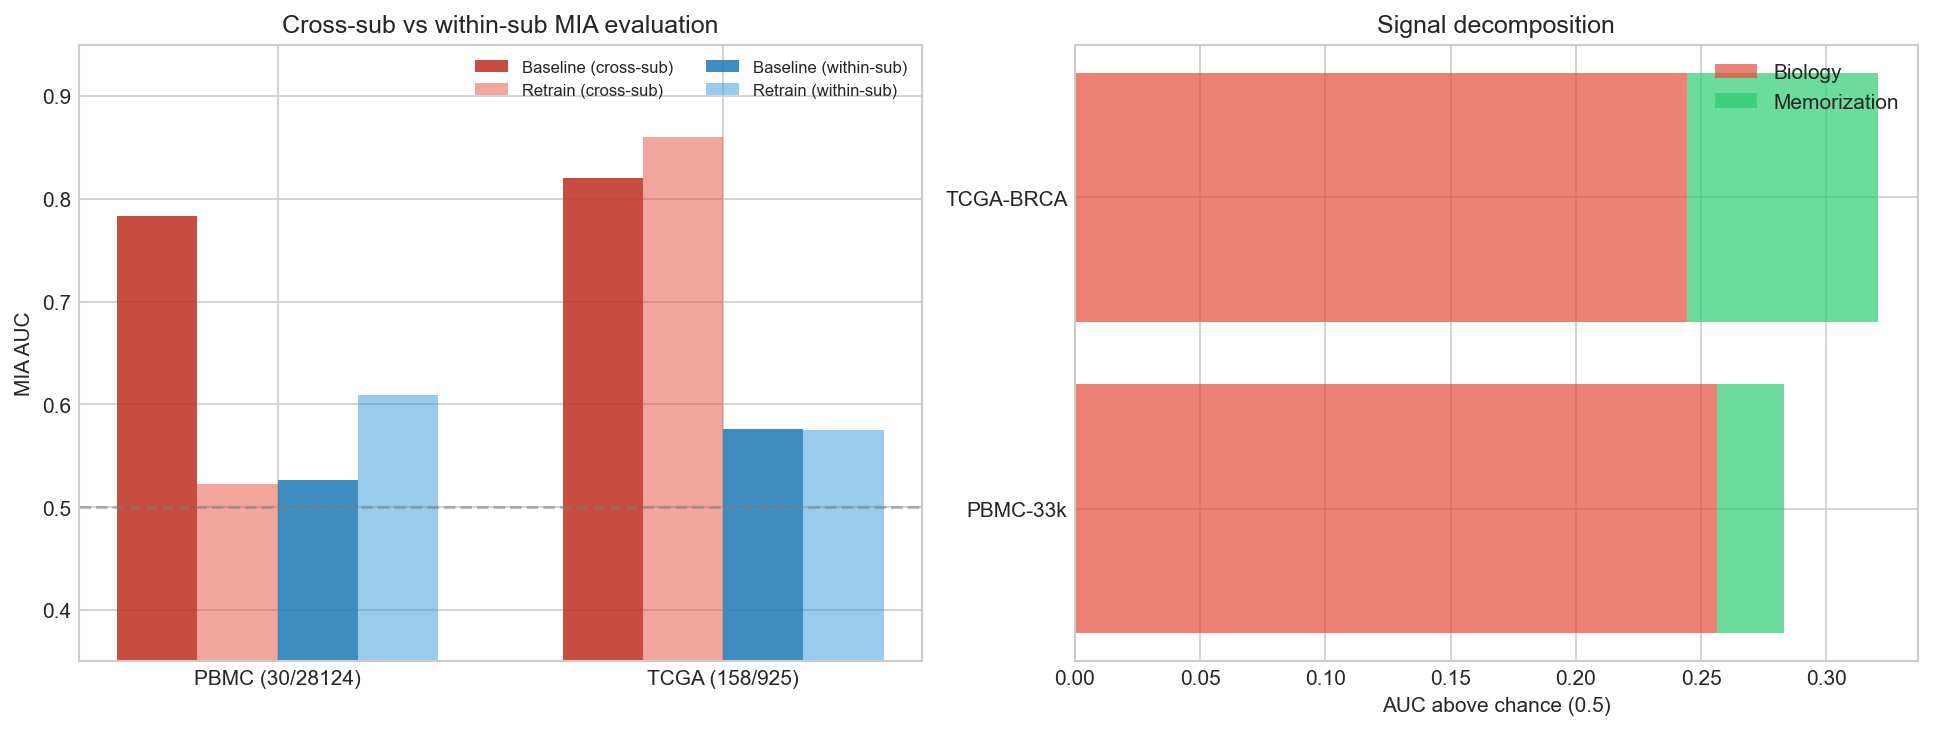
\includegraphics[width=0.95\textwidth]{figures/confound_comparison.png}
\caption{Biology confound across datasets. Left: cross-subtype vs.\ within-subtype MIA AUC for PBMC and TCGA-BRCA. With within-subtype matching, baseline and retrain AUCs converge. Right: decomposition of the cross-subtype AUC signal into biology (red) and memorization (green) components.}
\label{fig:confound}
\end{figure}

\section{Corollary 2 proof}
\label{app:corollary_proof}

(i) $\langle \sigma^{\mathcal{F}}, \sigma^{\mathcal{R}} \rangle \geq (D - M)\bar{\sigma}^2$ from the shared dimensions, while $\|\sigma^S\|^2 \leq (D-M)\bar{\sigma}^2 + M V^2 \bar{\sigma}^2$ for each set, giving the stated bound, which tends to $1$ as $D/M \to \infty$. (ii) For $\sigma^{\mathcal{F}} = \sigma^{\mathcal{F}}_k \mathbf{e}_k$ the cosine reduces to $\sigma^{\mathcal{R}}_k / \|\sigma^{\mathcal{R}}\|$, which equals $1/\sqrt{C}$ for balanced $C$-class residuals.\hfill$\square$

\section{Empirical verification of the factorization}
\label{app:empirical_verification}

The fc\_mean Fisher matrix is approximately rank-1, with the leading singular value explaining $98\%$ of the Frobenius norm for the forget set and $94\%$ for the retain set, consistent with the outer-product form $F_{dh} \approx 4\sigma_d\nu_h$ from Proposition~\ref{prop:factorization}. The Fisher-marginal factorization $\cos(\sigma^{\mathcal{F}}, \sigma^{\mathcal{R}}) \cdot \cos(\nu^{\mathcal{F}}, \nu^{\mathcal{R}}) = 0.50$ overshoots the measured cosine of $0.485$ by 3\%. The residual error comes from the softmax output Jacobian, which couples output dimensions and departs from the element-wise independence assumed in Proposition~\ref{prop:factorization}. Under the per-sample estimator both factors track their data-direct counterparts closely, with Fisher-marginal $\nu$ ($0.60$) against the data-direct value ($0.63$) and Fisher-marginal $\sigma$ ($0.83$) against the data-direct residual variance ($0.85$), and the product computed directly from data statistics ($0.53$) overshoots the measured cosine by 10\%. The $27\times$ gap in the shared output layer over the classifier ($0.485$ vs.\ $0.018$) is consistent with the structural prediction.

\section{Fisher overlap across datasets}
\label{app:fisher_crossdataset}

\begin{figure}[h]
\centering
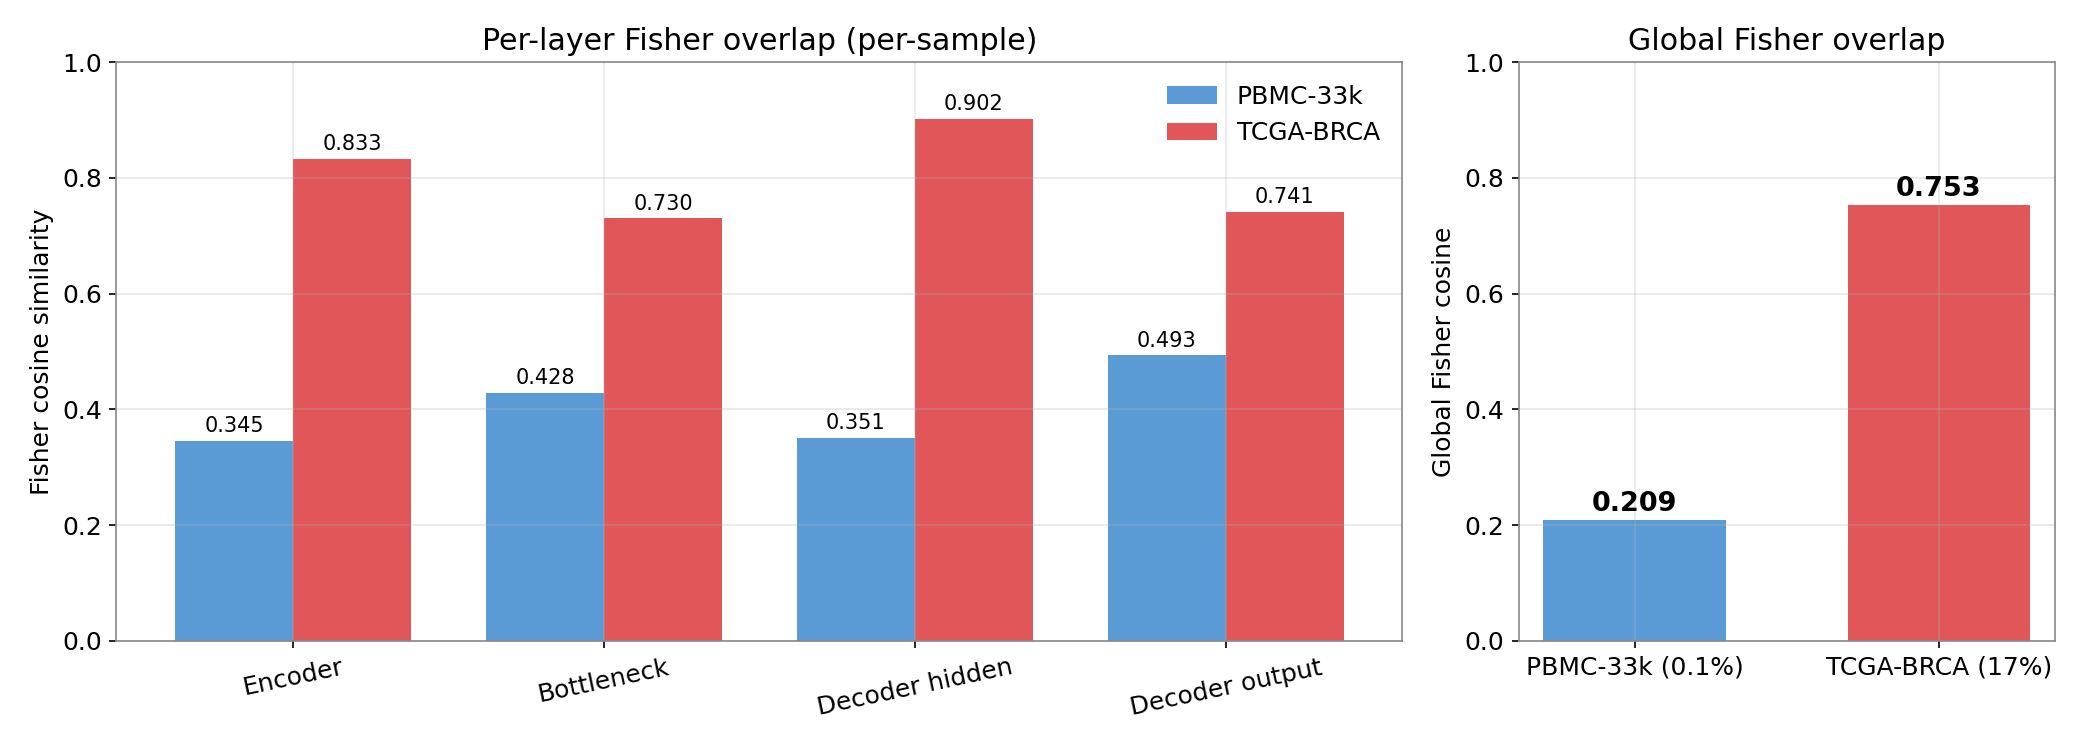
\includegraphics[width=0.85\textwidth]{figures/fisher_overlap_cross_dataset.png}
\caption{Fisher overlap on PBMC-33k (0.1\% forget fraction) versus TCGA-BRCA (17\%). Left: per-layer cosine. Right: global cosine. TCGA-BRCA overlap is uniformly higher, driven by the larger forget fraction and fewer output dimensions.}
\label{fig:fisher_crossdataset}
\end{figure}

\section{Cluster-conditional decoder}
\label{app:cvae}

A conditional VAE was trained in which the mean output layer receives the final hidden representation concatenated with a 14-dimensional cluster one-hot vector (adding 28K parameters). The fc\_mean weight matrix then decomposes into shared columns (corresponding to the 1,024 hidden features) and cluster-specific columns (corresponding to the 14 one-hot inputs). The shared columns have cosine $= 0.379$, reflecting irreducible overlap from the shared hidden representation. The cluster-specific columns have cosine $\approx 0$ ($5 \times 10^{-9}$), achieving the same near-orthogonality as the classifier output weights. Fisher scrubbing on this conditional VAE was applied with the same hyperparameters as the standard experiments. The conditional VAE baseline shows higher memorization (advantage $= 0.76$) than the standard VAE ($0.54$), likely because the cluster-specific columns give the model additional capacity to distinguish cluster~13. After scrubbing, advantage drops to $0.71$, a negligible reduction. Fisher overlap persists throughout the shared network with encoder cosine $= 0.62$, bottleneck $= 0.65$, and decoder hidden $= 0.51$. Since the MIA attacker draws 64 of its 70 feature dimensions from encoder outputs, the high encoder overlap is the dominant factor. Routing cluster-specific information through dedicated output parameters does not reduce memorization already encoded in the shared encoder and hidden layers.

\section{Cross-dataset validation}
\label{app:crossdataset}

\begin{table}[h]
\centering
\caption{Cross-dataset comparison (PBMC-33k vs.\ Tabula Muris). PBMC values use the single-seed attacker (baseline $= 0.769$, retrain $= 0.481$; cf.\ Table~\ref{tab:methods} multi-seed where baseline $= 0.791$, retrain $= 0.578$). The Tabula Muris retrain AUC ($0.944$) exceeds the baseline ($0.891$), so the TM attacker is measuring cell-type identifiability, not membership. $^\dagger$Fisher fails on PBMC (gap $0.241$ above multi-seed retrain) but is uninterpretable on TM where there is no membership signal to remove.}
\label{tab:crossdataset}
\begin{tabular}{lccccc}
\toprule
Method & \multicolumn{2}{c}{PBMC} & \multicolumn{2}{c}{Tabula Muris} & Gen.? \\
 & AUC & Baseline & AUC & Baseline & \\
\midrule
Retrain (structured) & 0.481 & 0.769 & 0.944 & 0.891 & -- \\
EG $\lambda=10$ (structured) & 0.482 & 0.769 & 0.874 & 0.891 & No \\
Fisher (structured) & 0.814 & 0.769 & 0.946 & 0.891 & PBMC fails$^\dagger$ \\
Fisher (scattered) & 0.499 & 0.525 & 0.568 & 0.411 & -- \\
\bottomrule
\end{tabular}
\end{table}

\section{Privacy-utility plane}
\label{app:tradeoff}

\begin{figure}[h]
\centering
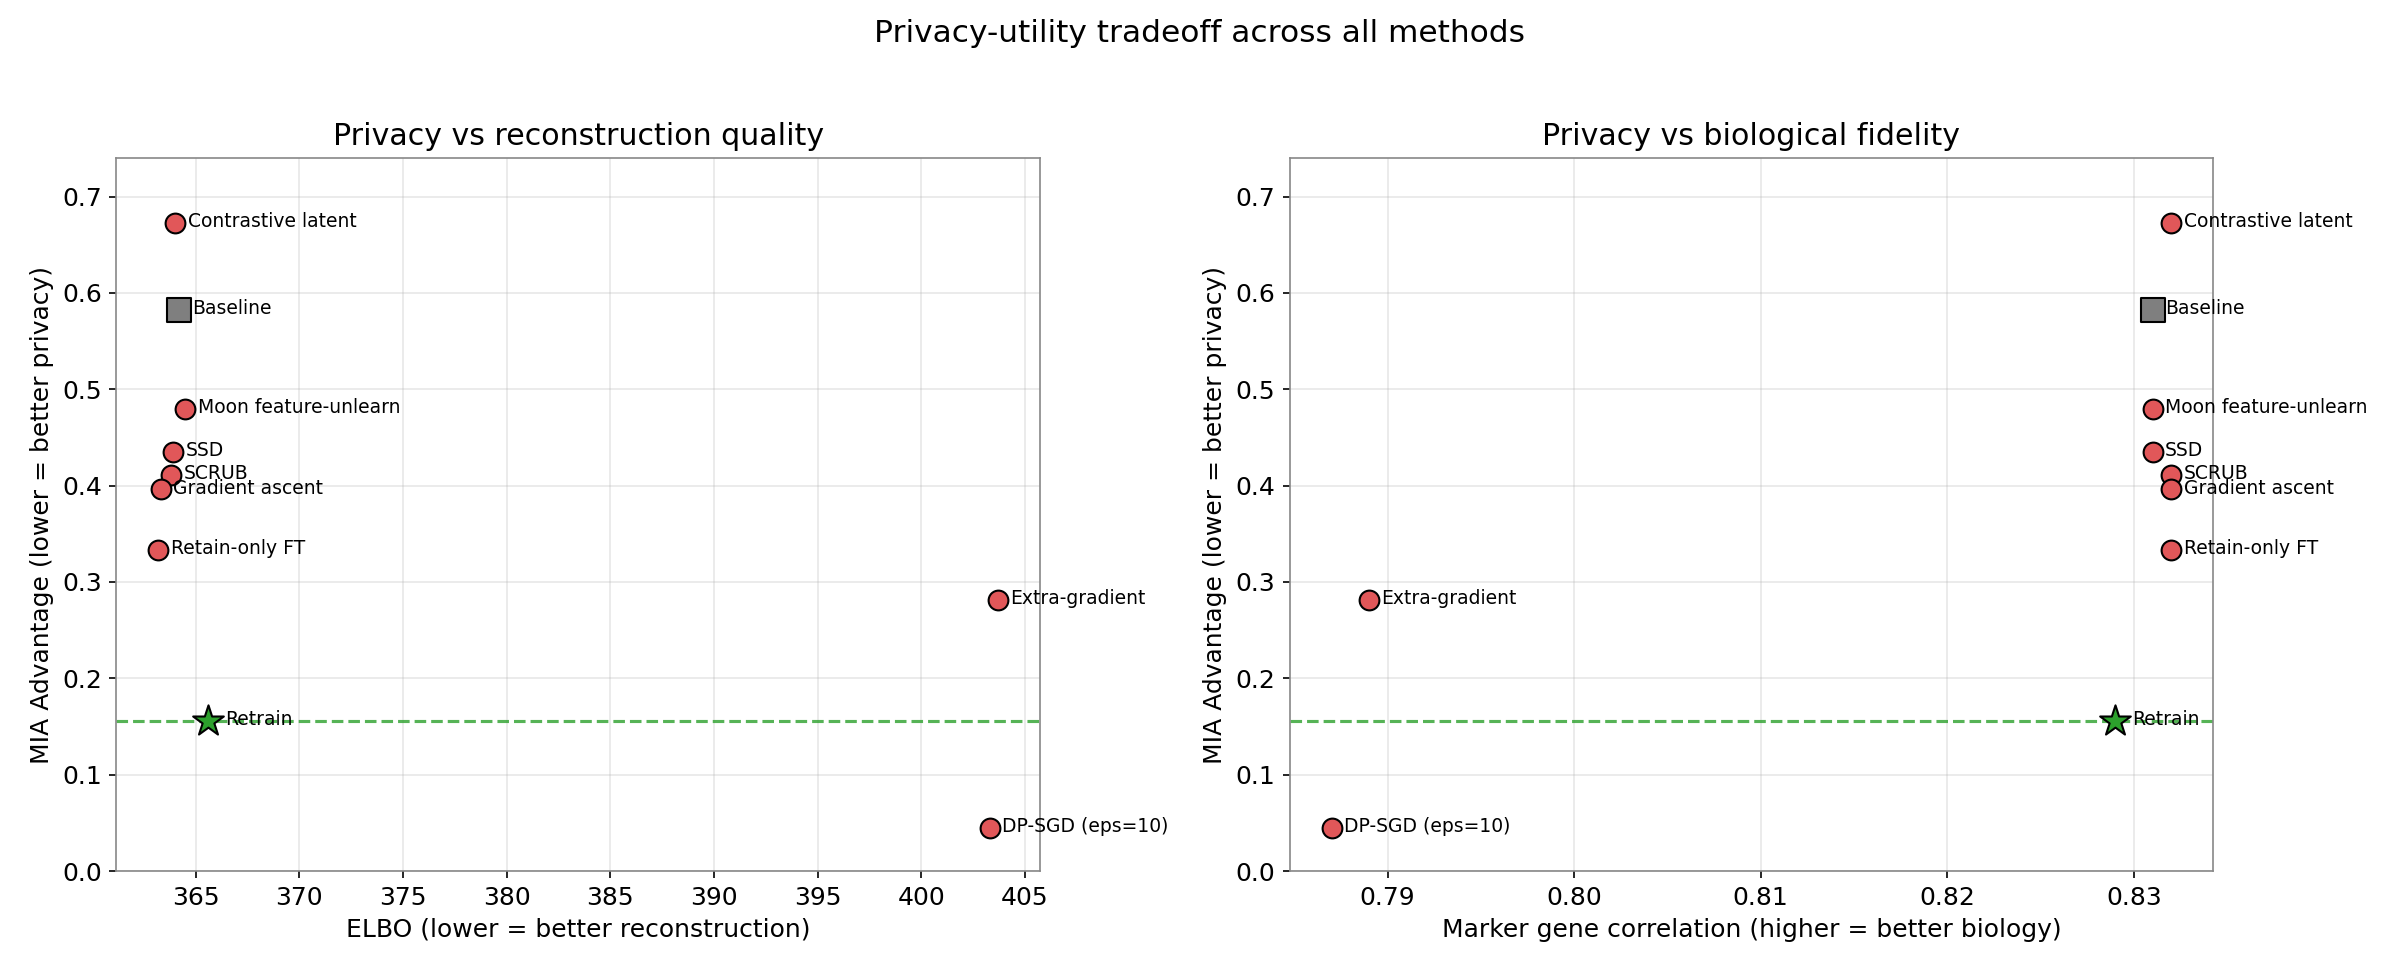
\includegraphics[width=0.85\textwidth]{figures/privacy_utility_all_methods.png}
\caption{Privacy-utility tradeoff across all methods. Left: advantage vs.\ ELBO. Right: advantage vs.\ marker gene correlation. Methods that preserve utility (upper cluster) fail on privacy; methods that reduce advantage (DP-SGD, extra-gradient) pay a utility cost. Only retrain achieves both.}
\label{fig:tradeoff}
\end{figure}

\section{Fisher unlearning on scattered forget sets}
\label{app:fisher_scattered}

Fisher scrubbing behaves differently by forget-set structure (Table~\ref{tab:fisher_type}). Scattered forget sets are near-chance at baseline (AUC $= 0.525$), and Fisher brings advantage to $\Delta = 0.026$ above baseline, a marginal improvement of cells that were barely memorized. On structured sets, the posterior collapses and advantage rises from $0.538$ to $0.628$. Fisher cannot reduce the signal where the signal exists.

\begin{table}[h]
\centering
\caption{Fisher unlearning on PBMC-33k by forget set type (3 seeds). Fisher reduces AUC on scattered sets, where baseline memorization is already weak. On structured sets it increases AUC through posterior collapse.}
\label{tab:fisher_type}
\begin{tabular}{lcccc}
\toprule
Forget type & Mean AUC & Std & Baseline AUC & Status \\
\midrule
Structured & 0.814 & 0.003 & 0.769 & FAIL (worse) \\
Scattered & 0.499 & 0.004 & 0.525 & At chance \\
\bottomrule
\end{tabular}
\end{table}

\begin{figure}[h]
\centering
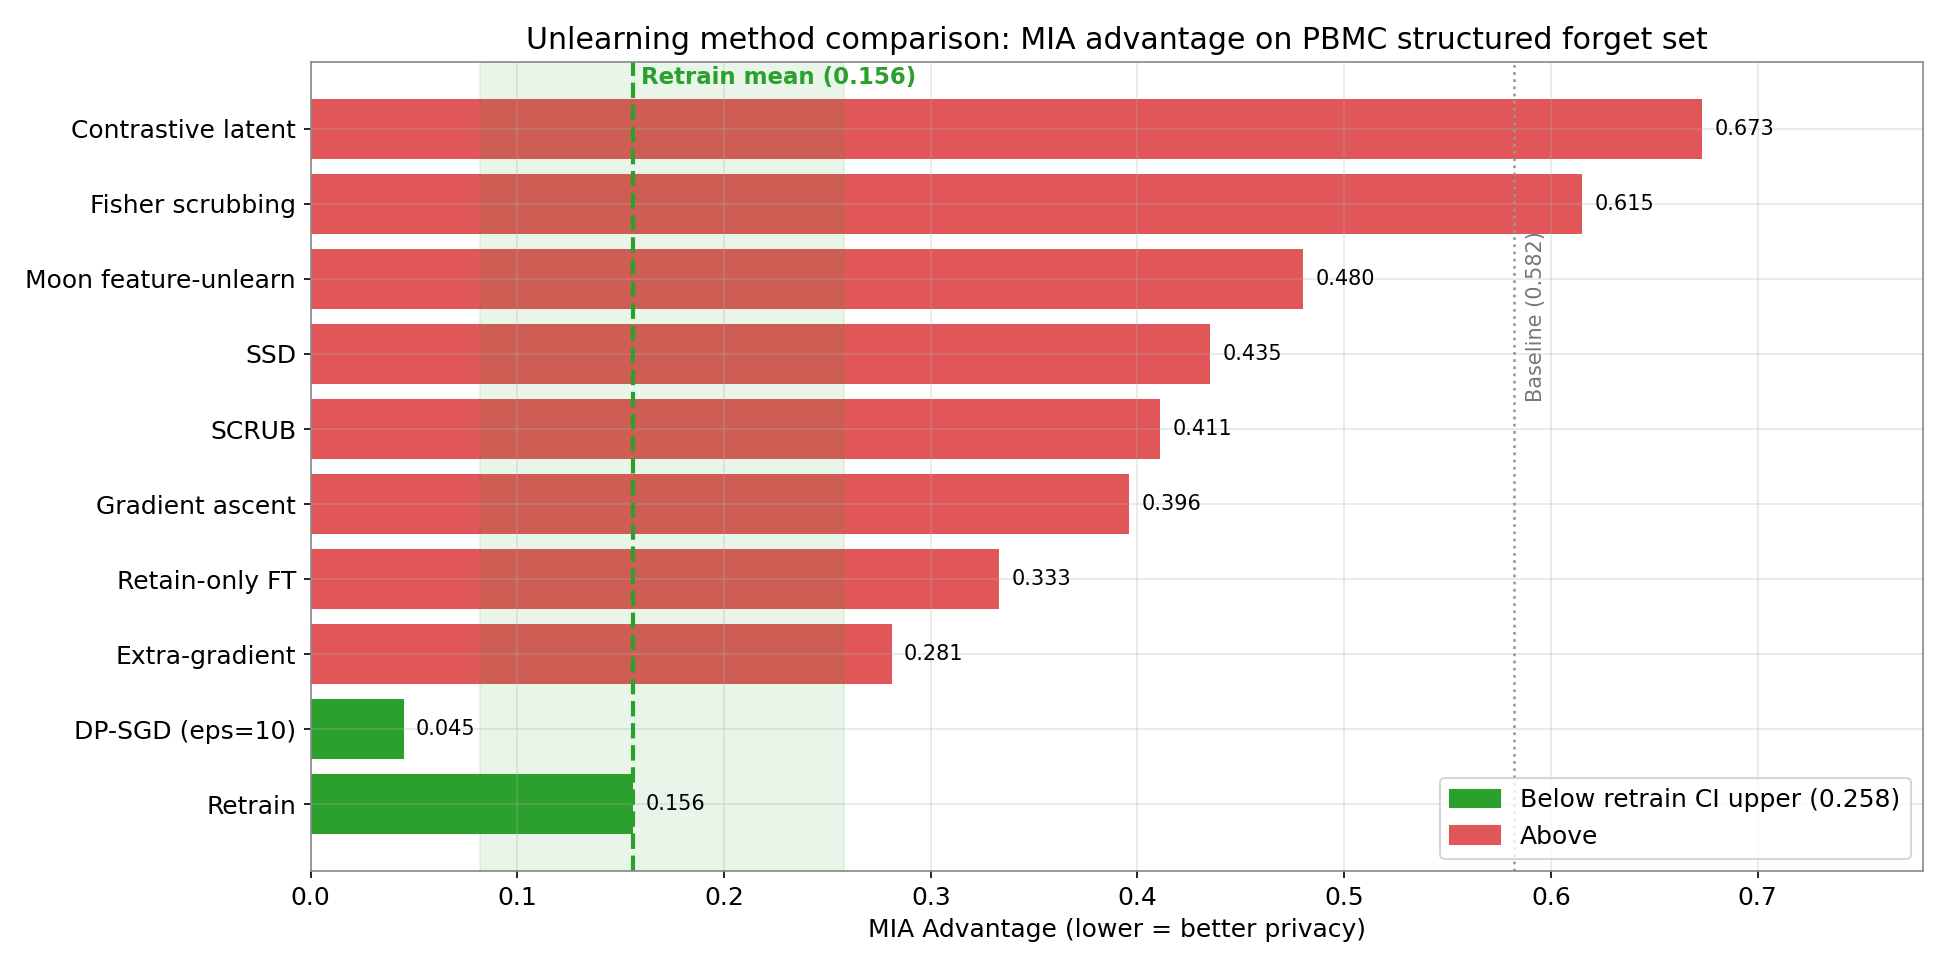
\includegraphics[width=0.85\textwidth]{figures/method_comparison_advantage.png}
\caption{MIA advantage by method on PBMC-33k structured forget set ($n=30$). The dashed line marks the 5-seed retrain advantage mean ($0.156$) with shaded nested 95\% CI $[0.082, 0.258]$. DP-SGD's advantage ($0.045$) is not distinguishable from retrain but trains from scratch. No post-hoc unlearning method's advantage-difference CI reaches zero.}
\label{fig:advantage}
\end{figure}

\section{Per-parameter Fisher scatter}
\label{app:fisher_scatter}

\begin{figure}[h]
\centering
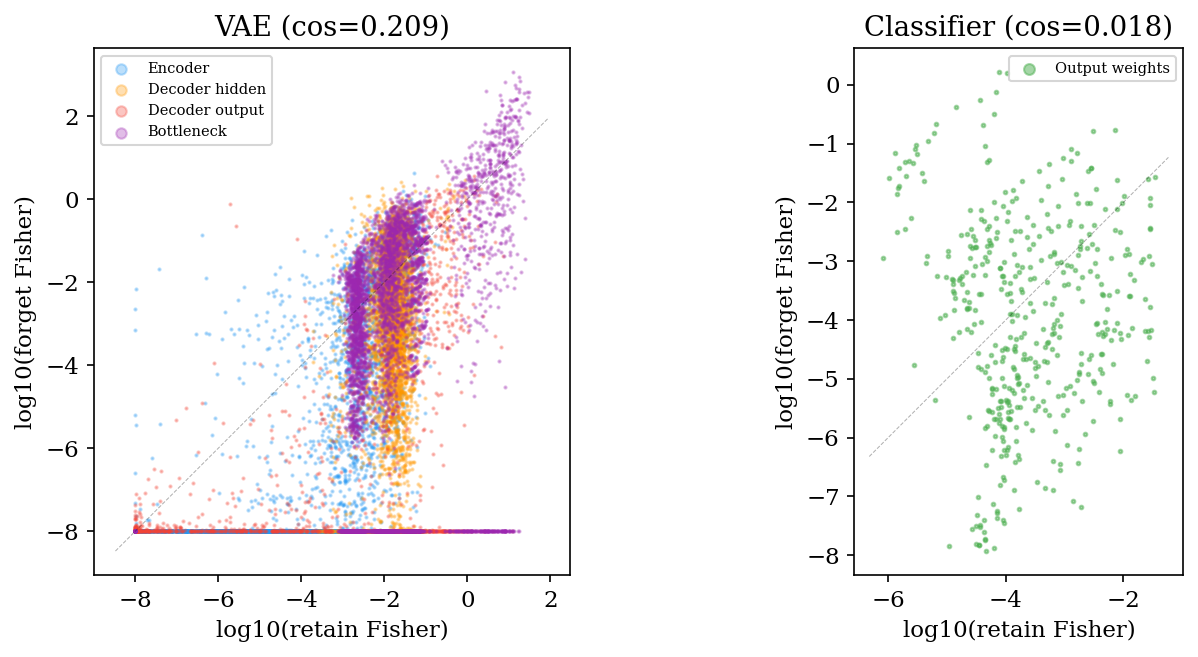
\includegraphics[width=0.95\textwidth]{figures/fisher_scatter.png}
\caption{Per-parameter Fisher magnitude (log scale) for forget vs.\ retain sets. Left: VAE parameters are correlated (log-Fisher $r = 0.71$), confirming that the same parameters matter for both sets. Right: classifier parameters show no correlation ($\cos = 0.018$), with forget-set Fisher concentrated in a few class-specific weights.}
\label{fig:fisher_scatter}
\end{figure}

\newpage

\end{document}
